\documentclass{report}
\usepackage[francais ]{babel}
\usepackage[utf8]{inputenc}
\usepackage[T1]{fontenc}
\usepackage{graphicx}
\usepackage{tabto}
\title{Spécifications techniques}
\author{M. \textsc{Friedli}, A. \textsc{Gillioz}, J. \textsc{Guerne}\\
He-Arc Ingénierie\\
2000 Neuchatel}
\date{\today{}}
\begin{document}
\maketitle{}
\chapter{Spécifications}
\section{Menu Application}
\subsection{Lancer application}
Lorsqu'un utilisateur lance l'application, il arrive dans le menu. A ce moment, il peut décider, soit de lancer une partie, soit de quitter l'application (Figure \ref{diagramme-mainApp}).
\begin{figure}[ht]
	\centering\includegraphics[width=9cm]{menuApplication}
	\caption{Diagramme des cas d'utilisations du menu}
	\label{diagramme-mainApp}
\end{figure}
\subsection{Lancer partie}
Quand l'utilisateur souhaite lancer une partie, il faut au préalable qu'il se connecte au serveur de jeu. Pour ce faire, il fait une demande de connexion audit serveur.
Si la connexion est réussit, le serveur l'ajoute à sa liste de client. Puis, le client indique quelle version de l'application il utilise.
Si sa version n'est pas la dernière, la connexion est refusée. Il reçoit un message d'erreur lui indiquant que sa version n'est pas à jour.
Autrement, la connexion est réussie (Figure \ref{diagramme-connexion}).
\begin{figure}[ht]
	\centering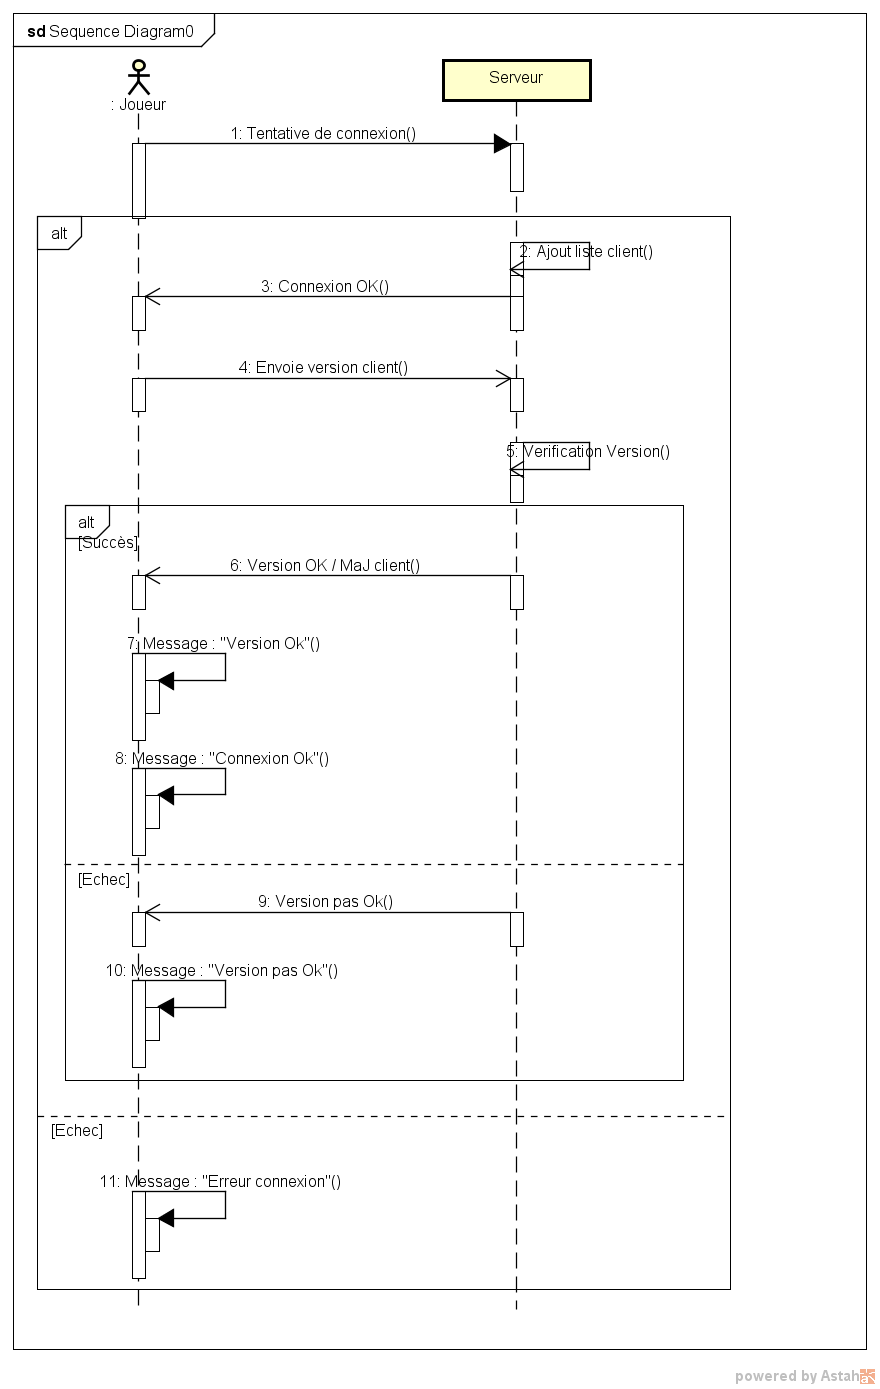
\includegraphics[width=10cm, height=13cm]{ConnexionServeur}
	\caption{Diagramme de séquence de la connexion}
	\label{diagramme-connexion}
\end{figure}
\subsection{Chercher un joueur}
Une fois que l'utilisateur est connecté au serveur, il choisit un jeu et l'indique au serveur ce dernier va l'ajouter à la liste des joueurs en attente et le prévenir
qu'il lui cherche un adversaire. Ensuite, il va tenter de trouver un autre joueur. Dès que c'est fait le serveur indique aux deux joueurs qu'une partie a été trouvée.
\subsection{quitter}
Quand l'utilisateur quitte l'application, il envoie un message au serveur qui le retire de sa liste de clients (basée selon le modèle de connexion/déconnexion du protocole TCP).
Puis, l'application se ferme.
\section{En jeu}
\subsection{Jouer/Action}
Une fois que la partie s'est lancé, le premier joueur (déterminé aléatoirement) fait son action côté client. Une fois ladite action effectué, elle est envoyée au serveur
qui va faire les calculs. Ensuite, il va communiquer aux deux clients les mises à jours de la partie (Figures \ref{diagramme-useCase-jeu} et \ref{diagramme-sequence-jeu}).
C'est à présent au deuxième joueur de jouer. \par
\begin{figure}[ht]
	\centering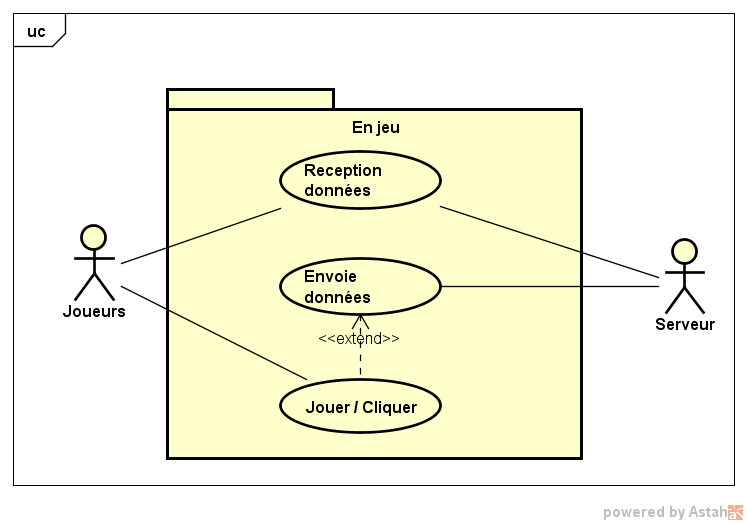
\includegraphics[width=9cm]{InGame}
	\caption{Diagramme des cas d'utilisation en jeu}
	\label{diagramme-useCase-jeu}
\end{figure}
\newpage
Le serveur gère également un temps d'exécution maximum pour le tour d'un joueur. Si ce temps est dépassé, le joueur perd son tour.
Si jamais le serveur reçoit l'information de la déconnexion d'un des joueurs, il quittra la partie.
Il est aussi chargé de vérifié si la partie est terminée et, le cas échéant, l'indique aux deux joueurs (victoire, défaite ou égalité)
\begin{figure}[ht]
	\centering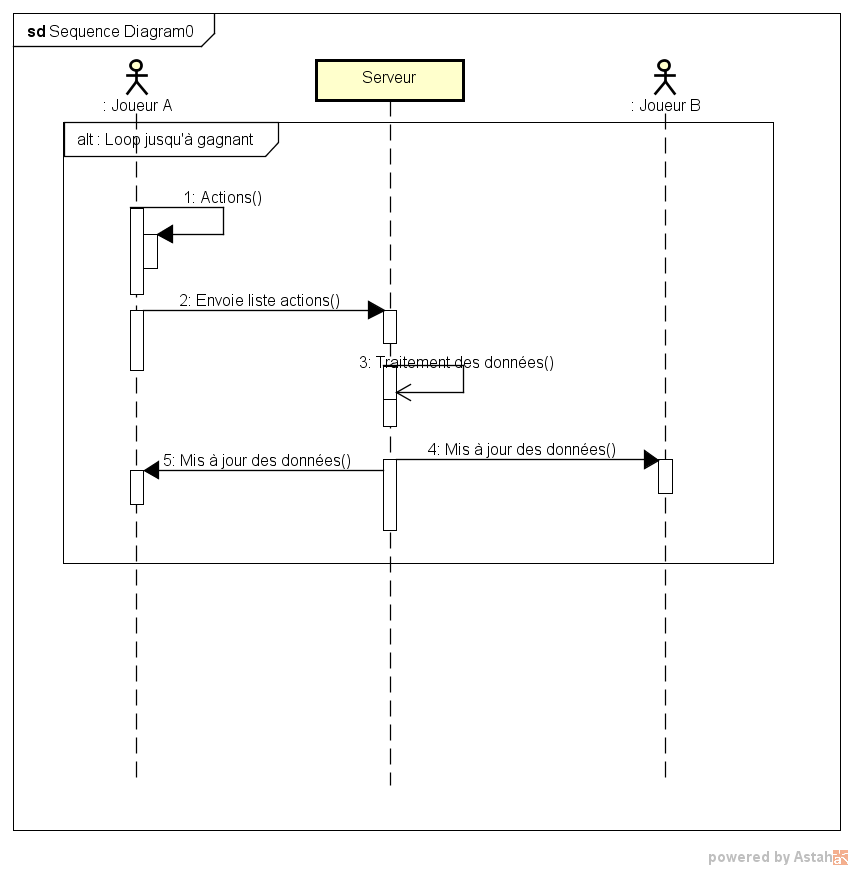
\includegraphics[width=9cm]{SequenceJeu}
	\caption{Diagramme de séquence d'une partie}
	\label{diagramme-sequence-jeu}
\end{figure}
\chapter{Conventions}
\section{convension de codage}
Les différentes conventions de codage présenté ci-dessous viennent principalement du site www.developpez.com.
La langue utilisé pour le codage (noms variables et noms des méthodes)  est l'anglais.
\subsection{Package}
Tout en minuscule. \\
Utiliser uniquement [a-z][0-9] et le point.
\subsection{Classes et interfaces}
Selon la norme PascalCase.
\subsection{Méthodes et attributs}
Selon la norme camelCase. \\
Les méthodes commencerront toujours par un verbe.
\subsection{Constantes}
Les variables déclarées en tant que constantes sont en majuscule et séparé par un \og \_ \fg{}.
\subsection{paramètres des fonctions}
Selon la norme camelCase.
\subsection{Identation}
Les accolades sont déclarées sous l’instruction précédent le bloc.\\
La première instruction du bloc est décalée et l’indentation générale est de un \og tab \fg{}.

\section{id des paquets}
Tous les paquets qui circulent lors du déroulement d'un jeu ont un id qui doit respecter la convension suivante :
\begin{itemize}
	\item Morpion \tabto{4cm} 1000 à 1999
	\item Bataille navale \tabto{4cm} 2000 à 2999
	\item Jeu de dames \tabto{4cm} 3000 à 3999
\end{itemize}
\section{Morpion}
Les coordonnées du morpion seront représentées par une matrice 3x3 qui sera implémentée par une liste de liste.
Le remplissage d'une case respectera la convension suivante :
\begin{itemize}
	\item case vide \tabto{4cm} chiffre 0
	\item case joueur 1 \tabto{4cm} chiffre 1
	\item case joueur 2 \tabto{4cm} chiffre 2
\end{itemize}
\section{Bataille navalle}
Les coordonnées d'un plateau de baitaille navale seront représentées par une matrice 10x10. Sachant qu'il faut deux plateaux (un pour le joueur, l'autre pour l'adversaire),
nous aurons donc deux implémentations de liste de liste.
Le plateau du joueur respectera la convension suivante :
\begin{itemize}
	\item case sans bateau \tabto{4cm} chiffre 0
	\item case avec bateau \tabto{4cm} chiffre 1
\end{itemize}
Le plateau du joueur adverse respectera la consention suivante :
\begin{itemize}
	\item case non explorée \tabto{4cm} chiffre 0
	\item case explorée \og à l'eau \fg{} \tabto{4cm} chiffre 1
	\item case explorée \og touché \fg{} \tabto{4cm} chiffre 2
\end{itemize}
\section{Jeu de Dames}
Les coordonnées d'un plateau de jeu de Dames seront représentées par une matrice 8x8 qui sera implémentée par une liste de liste.
Le remplissage d'une case restepectera la convesion suivante :
\begin{itemize}
	\item case vide \tabto{4cm} chiffre 0
	\item pion joueur 1 \tabto{4cm} chiffre 1
	\item pion joueur 2  \tabto{4cm} chiffre 2
	\item dame joueur 1 \tabto{4cm} chiffre 3
	\item damte joueur 2 \tabto{4cm} chiffre 4
\end{itemize}

\chapter{Objectifs}
Cette partie décrit les principaux objectifs que nous nous sommes fixés.
\section{Objectifs}\label{objectifs}
\begin{itemize}
	\item Faire communiquer un client avec un serveur.
	\item Le serveur renvera ensuite les données demandé par le client.
	\item Créer des mini-jeux.
	\item Faire communiquer les clients entre eux via le serveur.
	\item Sérializer les données des jeux pour permettre le jeu en ligne.
	\item Le serveur fera la synchronisation des clients.
\end{itemize}
\section{Objectifs bonus}\label{objectifs-bonus}
\begin{itemize}
	\item Rechercher automatiquement les joueurs connectés à l'application.
\end{itemize}
\chapter{Description du projet}\label{desciption-projet}
Ce chapitre présente les différentes phases du programme. En expliquant l'architecture client/serveur que nous allons utiliser. La figure montre un schéma de notre
structure réseau.
\section{Maquette du projet}\label{maquette}


\end{document}
